\documentclass[11pt]{article}

\usepackage{graphicx}
\usepackage{amssymb,amsmath}
\usepackage{textcomp}

%\usepackage{subcaption}
%\usepackage{float}
\usepackage{setspace}
\usepackage{fullpage}
\usepackage[font=scriptsize]{caption}
%\usepackage{fullpage}
%\setcounter{secnumdepth}{1}
\begin{document}

\title{Pattern adaptation and normalization reweighting}
\author{Kari Y. Lam, Zachary M. Westrick, Others TBA}
\maketitle

\begin{abstract}
I'm MC Zack and I've got something to say. Hey. Hey. Hey. Hey. Hey
\end{abstract}

\section{Introduction}

\begin{figure}
\begin{center}
  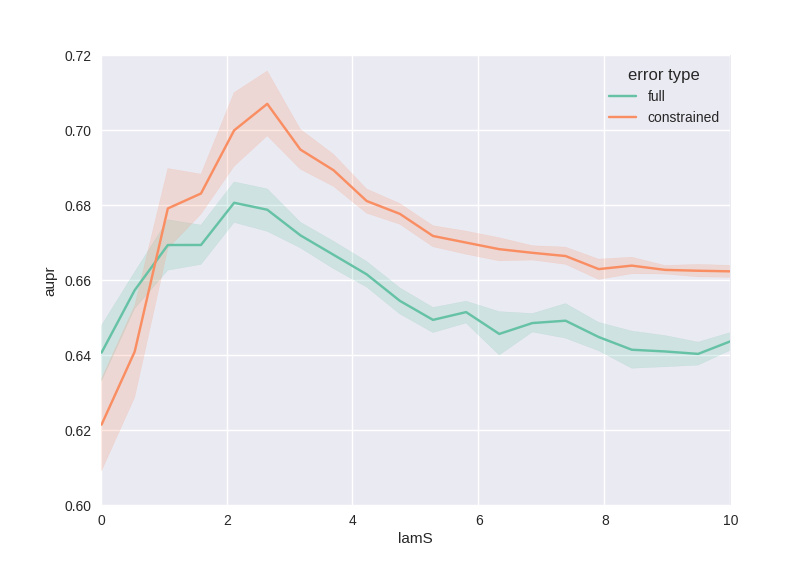
\includegraphics[scale=0.45]{simulated.png}
  \caption{\label{fig:figure1} This is what a figure looks like}
  \end{center}
\end{figure}

\section{Methods}
Look an equation array
\begin{equation}
\begin{array}{l}
R_i^{\mathrm{input}}(\theta) = c g_i^{\mathrm{input}}\exp(-(\theta - \theta_i)^2 / (2\sigma^2_{\mathrm{input}}))
\\
R_i^{\mathrm{output}}(\theta) = g_i^{\mathrm{output}}\sum_{j=0}^N R_j^{\mathrm{input}}(\theta) \exp(-(\theta_i - \theta_j)^2/(2\sigma^2_{\mathrm{output}})) .
\end{array}
\end{equation}
\bibliographystyle{plain}
\bibliography{paper}

\end{document}

